\documentclass[12pt,twoside,openany]{memoir}
\usepackage[T1]{fontenc}
%\usepackage{tgpagella} % text only
%\usepackage{mathpazo}  % math & text
\usepackage[T1]{fontenc}
\usepackage[hidelinks]{hyperref}
\usepackage{amsmath}
\usepackage{amsthm}
\usepackage{amssymb}
\usepackage{mathtools}
\usepackage{graphicx}
%\usepackage{newpxtext}
%\usepackage{eulerpx}
%\usepackage{eucal}
\usepackage{datetime}
    \newdateformat{specialdate}{\THEYEAR\ \monthname\ \THEDAY}
\usepackage[margin=1in]{geometry}
\usepackage{fancyhdr}
    \fancyhf{}
    \pagestyle{fancy}
    \cfoot{\scriptsize \thepage}
    \fancyhead[R]{\scriptsize \rightmark}
    \fancyhead[L]{\scriptsize \leftmark}
    \renewcommand{\headrulewidth}{0pt}
    \renewcommand{\footrulewidth}{0pt} % if you also want to remove the footer rule
\usepackage{mdframed}
\usepackage{pdfpages}
\mdfsetup{font=\small}

\mdfdefinestyle{mystyle}{linecolor=black }







\usepackage{thmtools}
    \declaretheoremstyle[
        spaceabove=10pt,
        spacebelow=10pt,
        headfont=\normalfont\bfseries,
        notefont=\mdseries, notebraces={(}{)},
        bodyfont=\normalfont,
        postheadspace=0.5em
        %qed=\qedsymbol
        ]{defs}

    \declaretheoremstyle[ 
        spaceabove=10pt, % space above the theorem
        spacebelow=10pt,
        headfont=\normalfont\bfseries,
        bodyfont=\normalfont\itshape,
        postheadspace=0.5em
        ]{thmstyle}
    
    \declaretheorem[
        style=thmstyle,
        numberwithin=section
    ]{theorem}

    \declaretheorem[
        style=thmstyle,
        sibling=theorem,
    ]{proposition}

    \declaretheorem[
        style=thmstyle,
        sibling=theorem,
    ]{lemma}

    \declaretheorem[
        style=thmstyle,
        sibling=theorem,
    ]{corollary}

    \declaretheorem[
        numberwithin=section,
        style=defs,
    ]{example}

    \declaretheorem[
        numberwithin=section,
        style=defs,
    ]{definition}

    \declaretheorem[
        style=defs,
        numbered=unless unique,
    ]{problem}

    \declaretheorem[
        numbered=unless unique,
        shaded={rulecolor=black,
    rulewidth=1pt, bgcolor={rgb}{1,1,1}}
    ]{axiom}

    \declaretheorem[numberwithin=section,style=defs]{note}
    \declaretheorem[numbered=no,style=defs]{question}
    \declaretheorem[numbered=no,style=defs]{recall}
    \declaretheorem[numbered=no,style=remark]{answer}
    \declaretheorem[numbered=no,style=remark]{solution}

    \declaretheorem[numbered=no,style=defs]{remark}
\usepackage{enumitem}
\usepackage{titlesec}
    \titleformat{\chapter}[display]
    {\bfseries\LARGE\raggedright}
    {Chapter {\thechapter}}
    {1ex minus .1ex}
    {\Huge}
    \titlespacing{\chapter}
    {3pc}{*3}{40pt}[3pc]

    \titleformat{\section}[block]
    {\normalfont\bfseries\Large}
    {\S\ \thesection.}{.5em}{}[]
    \titlespacing{\section}
    {0pt}{3ex plus .1ex minus .2ex}{3ex plus .1ex minus .2ex}
\usepackage[utf8x]{inputenc}
\usepackage{tikz}
\usepackage{tikz-cd}
\usepackage{wasysym}
\usepackage{pgf}
\usepackage{mmacells}
\usepackage{listings}
\usepackage{xcolor}

\definecolor{codegreen}{rgb}{0,0.6,0}
\definecolor{codegray}{rgb}{0.5,0.5,0.5}
\definecolor{codepurple}{rgb}{0.58,0,0.82}
\definecolor{backcolour}{rgb}{0.95,0.95,0.92}

\lstdefinestyle{mystyle}{
    backgroundcolor=\color{backcolour},   
    commentstyle=\color{codegreen},
    keywordstyle=\color{magenta},
    numberstyle=\tiny\color{codegray},
    stringstyle=\color{codepurple},
    basicstyle=\ttfamily\footnotesize,
    breakatwhitespace=false,         
    breaklines=true,                 
    captionpos=b,                    
    keepspaces=true,                 
    numbers=left,                    
    numbersep=5pt,                  
    showspaces=false,                
    showstringspaces=false,
    showtabs=false,                  
    tabsize=2
}

\lstset{style=mystyle}
\usepackage{fancyvrb}
\usepackage{tcolorbox}

% Define replacements: "what to look for" => "how to typeset it"
\mmaDefineMathReplacement[≤]{<=}{\leq}
\mmaDefineMathReplacement[≥]{>=}{\geq}
\mmaDefineMathReplacement[≠]{!=}{\neq}
\mmaDefineMathReplacement[→]{->}{\to}[2]
\mmaDefineMathReplacement[⧴]{:>}{:\hspace{-.2em}\to}[2]
\mmaDefineMathReplacement{∉}{\notin}
\mmaDefineMathReplacement{∞}{\infty}
\mmaDefineMathReplacement{𝕕}{\mathbbm{d}}

\linespread{1}
%to make the correct symbol for Sha
%\newcommand\cyr{%
%\renewcommand\rmdefault{wncyr}%
%\renewcommand\sfdefault{wncyss}%
%\renewcommand\encodingdefault{OT2}%
%\normalfont \selectfont} \DeclareTextFontCommand{\textcyr}{\cyr}


\DeclareMathOperator{\ab}{ab}
\newcommand{\absgal}{\G_{\bbQ}}
\DeclareMathOperator{\ad}{ad}
\DeclareMathOperator{\adj}{adj}
\DeclareMathOperator{\alg}{alg}
\DeclareMathOperator{\Alt}{Alt}
\DeclareMathOperator{\Ann}{Ann}
\DeclareMathOperator{\arith}{arith}
\DeclareMathOperator{\Aut}{Aut}
\DeclareMathOperator{\Be}{B}
\DeclareMathOperator{\Bd}{Bd}
\DeclareMathOperator{\card}{card}
\DeclareMathOperator{\Char}{char}
\DeclareMathOperator{\csp}{csp}
\DeclareMathOperator{\codim}{codim}
\DeclareMathOperator{\coker}{coker}
\DeclareMathOperator{\coh}{H}
\DeclareMathOperator{\compl}{compl}
\DeclareMathOperator{\conj}{conj}
\DeclareMathOperator{\cont}{cont}
\DeclareMathOperator{\Cov}{Cov}
\DeclareMathOperator{\crys}{crys}
\DeclareMathOperator{\Crys}{Crys}
\DeclareMathOperator{\cusp}{cusp}
\DeclareMathOperator{\diag}{diag}
\DeclareMathOperator{\diam}{diam}
\DeclareMathOperator{\Dom}{Dom}
\DeclareMathOperator{\disc}{disc}
\DeclareMathOperator{\dist}{dist}
\DeclareMathOperator{\dR}{dR}
\DeclareMathOperator{\Eis}{Eis}
\DeclareMathOperator{\End}{End}
\DeclareMathOperator{\ev}{ev}
\DeclareMathOperator{\eval}{eval}
\DeclareMathOperator{\Eq}{Eq}
\DeclareMathOperator{\Ext}{Ext}
\DeclareMathOperator{\Fil}{Fil}
\DeclareMathOperator{\Fitt}{Fitt}
\DeclareMathOperator{\Frob}{Frob}
\DeclareMathOperator{\G}{G}
\DeclareMathOperator{\Gal}{Gal}
\DeclareMathOperator{\GL}{GL}
\DeclareMathOperator{\Gr}{Gr}
\DeclareMathOperator{\Graph}{Graph}
\DeclareMathOperator{\GSp}{GSp}
\DeclareMathOperator{\GUn}{GU}
\DeclareMathOperator{\Hom}{Hom}
\DeclareMathOperator{\id}{id}
\DeclareMathOperator{\Id}{Id}
\DeclareMathOperator{\Ik}{Ik}
\DeclareMathOperator{\IM}{Im}
\DeclareMathOperator{\Image}{im}
\DeclareMathOperator{\Ind}{Ind}
\DeclareMathOperator{\Inf}{inf}
\DeclareMathOperator{\Isom}{Isom}
\DeclareMathOperator{\J}{J}
\DeclareMathOperator{\Jac}{Jac}
\DeclareMathOperator{\lcm}{lcm}
\DeclareMathOperator{\length}{length}
\DeclareMathOperator*{\limit}{limit}
\DeclareMathOperator{\Log}{Log}
\DeclareMathOperator{\M}{M}
\DeclareMathOperator{\Mat}{Mat}
\DeclareMathOperator{\N}{N}
\DeclareMathOperator{\Nm}{Nm}
\DeclareMathOperator{\NIk}{N-Ik}
\DeclareMathOperator{\NSK}{N-SK}
\DeclareMathOperator{\new}{new}
\DeclareMathOperator{\obj}{obj}
\DeclareMathOperator{\old}{old}
\DeclareMathOperator{\ord}{ord}
\DeclareMathOperator{\Or}{O}
\DeclareMathOperator{\op}{op}
\DeclareMathOperator{\PGL}{PGL}
\DeclareMathOperator{\PGSp}{PGSp}
\DeclareMathOperator{\rank}{rank}
\DeclareMathOperator{\Ran}{Ran}
\DeclareMathOperator{\Rel}{Rel}
\DeclareMathOperator{\Real}{Re}
\DeclareMathOperator{\RES}{res}
\DeclareMathOperator{\Res}{Res}
%\DeclareMathOperator{\Sha}{\textcyr{Sh}}
\DeclareMathOperator{\Sel}{Sel}
\DeclareMathOperator{\semi}{ss}
\DeclareMathOperator{\sgn}{sign}
\DeclareMathOperator{\SK}{SK}
\DeclareMathOperator{\SL}{SL}
\DeclareMathOperator{\SO}{SO}
\DeclareMathOperator{\Sp}{Sp}
\DeclareMathOperator{\Span}{span}
\DeclareMathOperator{\Spec}{Spec}
\DeclareMathOperator{\spin}{spin}
\DeclareMathOperator{\st}{st}
\DeclareMathOperator{\St}{St}
\DeclareMathOperator{\SUn}{SU}
\DeclareMathOperator{\supp}{supp}
\DeclareMathOperator{\Sup}{sup}
\DeclareMathOperator{\Sym}{Sym}
\DeclareMathOperator{\Tam}{Tam}
\DeclareMathOperator{\tors}{tors}
\DeclareMathOperator{\tr}{tr}
\DeclareMathOperator{\Tr}{Tr}
\DeclareMathOperator{\un}{un}
\DeclareMathOperator{\Un}{U}
\DeclareMathOperator{\val}{val}
\DeclareMathOperator{\vol}{vol}

\DeclareMathOperator{\Sets}{S \mkern1.04mu e \mkern1.04mu t \mkern1.04mu s}
    \newcommand{\cSets}{\scalebox{1.02}{\contour{black}{$\Sets$}}}
    
\DeclareMathOperator{\Groups}{G \mkern1.04mu r \mkern1.04mu o \mkern1.04mu u \mkern1.04mu p \mkern1.04mu s}
    \newcommand{\cGroups}{\scalebox{1.02}{\contour{black}{$\Groups$}}}

\DeclareMathOperator{\TTop}{T \mkern1.04mu o \mkern1.04mu p}
    \newcommand{\cTop}{\scalebox{1.02}{\contour{black}{$\TTop$}}}

\DeclareMathOperator{\Htp}{H \mkern1.04mu t \mkern1.04mu p}
    \newcommand{\cHtp}{\scalebox{1.02}{\contour{black}{$\Htp$}}}

\DeclareMathOperator{\Mod}{M \mkern1.04mu o \mkern1.04mu d}
    \newcommand{\cMod}{\scalebox{1.02}{\contour{black}{$\Mod$}}}

\DeclareMathOperator{\Ab}{A \mkern1.04mu b}
    \newcommand{\cAb}{\scalebox{1.02}{\contour{black}{$\Ab$}}}

\DeclareMathOperator{\Rings}{R \mkern1.04mu i \mkern1.04mu n \mkern1.04mu g \mkern1.04mu s}
    \newcommand{\cRings}{\scalebox{1.02}{\contour{black}{$\Rings$}}}

\DeclareMathOperator{\ComRings}{C \mkern1.04mu o \mkern1.04mu m \mkern1.04mu R \mkern1.04mu i \mkern1.04mu n \mkern1.04mu g \mkern1.04mu s}
    \newcommand{\cComRings}{\scalebox{1.05}{\contour{black}{$\ComRings$}}}

\DeclareMathOperator{\hHom}{H \mkern1.04mu o \mkern1.04mu m}
    \newcommand{\cHom}{\scalebox{1.02}{\contour{black}{$\hHom$}}}

\renewcommand{\k}{\kappa}
\newcommand{\Ff}{F_{f}}
%\newcommand{\ts}{\,^{t}\!}


%Mathcal
\newcommand{\cA}{\mathcal{A}}
\newcommand{\cB}{\mathcal{B}}
\newcommand{\cC}{\mathcal{C}}
\newcommand{\cD}{\mathcal{D}}
\newcommand{\cE}{\mathcal{E}}
\newcommand{\cF}{\mathcal{F}}
\newcommand{\cG}{\mathcal{G}}
\newcommand{\cH}{\mathcal{H}}
\newcommand{\cI}{\mathcal{I}}
\newcommand{\cJ}{\mathcal{J}}
\newcommand{\cK}{\mathcal{K}}
\newcommand{\cL}{\mathcal{L}}
\newcommand{\cM}{\mathcal{M}}
\newcommand{\cN}{\mathcal{N}}
\newcommand{\cO}{\mathcal{O}}
\newcommand{\cP}{\mathcal{P}}
\newcommand{\cQ}{\mathcal{Q}}
\newcommand{\cR}{\mathcal{R}}
\newcommand{\cS}{\mathcal{S}}
\newcommand{\cT}{\mathcal{T}}
\newcommand{\cU}{\mathcal{U}}
\newcommand{\cV}{\mathcal{V}}
\newcommand{\cW}{\mathcal{W}}
\newcommand{\cX}{\mathcal{X}}
\newcommand{\cY}{\mathcal{Y}}
\newcommand{\cZ}{\mathcal{Z}}


%mathfrak (missing \fi)
\newcommand{\fa}{\mathfrak{a}}
\newcommand{\fA}{\mathfrak{A}}
\newcommand{\fb}{\mathfrak{b}}
\newcommand{\fB}{\mathfrak{B}}
\newcommand{\fc}{\mathfrak{c}}
\newcommand{\fC}{\mathfrak{C}}
\newcommand{\fd}{\mathfrak{d}}
\newcommand{\fD}{\mathfrak{D}}
\newcommand{\fe}{\mathfrak{e}}
\newcommand{\fE}{\mathfrak{E}}
\newcommand{\ff}{\mathfrak{f}}
\newcommand{\fF}{\mathfrak{F}}
\newcommand{\fg}{\mathfrak{g}}
\newcommand{\fG}{\mathfrak{G}}
\newcommand{\fh}{\mathfrak{h}}
\newcommand{\fH}{\mathfrak{H}}
\newcommand{\fI}{\mathfrak{I}}
\newcommand{\fj}{\mathfrak{j}}
\newcommand{\fJ}{\mathfrak{J}}
\newcommand{\fk}{\mathfrak{k}}
\newcommand{\fK}{\mathfrak{K}}
\newcommand{\fl}{\mathfrak{l}}
\newcommand{\fL}{\mathfrak{L}}
\newcommand{\fm}{\mathfrak{m}}
\newcommand{\fM}{\mathfrak{M}}
\newcommand{\fn}{\mathfrak{n}}
\newcommand{\fN}{\mathfrak{N}}
\newcommand{\fo}{\mathfrak{o}}
\newcommand{\fO}{\mathfrak{O}}
\newcommand{\fp}{\mathfrak{p}}
\newcommand{\fP}{\mathfrak{P}}
\newcommand{\fq}{\mathfrak{q}}
\newcommand{\fQ}{\mathfrak{Q}}
\newcommand{\fr}{\mathfrak{r}}
\newcommand{\fR}{\mathfrak{R}}
\newcommand{\fs}{\mathfrak{s}}
\newcommand{\fS}{\mathfrak{S}}
\newcommand{\ft}{\mathfrak{t}}
\newcommand{\fT}{\mathfrak{T}}
\newcommand{\fu}{\mathfrak{u}}
\newcommand{\fU}{\mathfrak{U}}
\newcommand{\fv}{\mathfrak{v}}
\newcommand{\fV}{\mathfrak{V}}
\newcommand{\fw}{\mathfrak{w}}
\newcommand{\fW}{\mathfrak{W}}
\newcommand{\fx}{\mathfrak{x}}
\newcommand{\fX}{\mathfrak{X}}
\newcommand{\fy}{\mathfrak{y}}
\newcommand{\fY}{\mathfrak{Y}}
\newcommand{\fz}{\mathfrak{z}}
\newcommand{\fZ}{\mathfrak{Z}}


%mathbf
\newcommand{\bfA}{\mathbf{A}}
\newcommand{\bfB}{\mathbf{B}}
\newcommand{\bfC}{\mathbf{C}}
\newcommand{\bfD}{\mathbf{D}}
\newcommand{\bfE}{\mathbf{E}}
\newcommand{\bfF}{\mathbf{F}}
\newcommand{\bfG}{\mathbf{G}}
\newcommand{\bfH}{\mathbf{H}}
\newcommand{\bfI}{\mathbf{I}}
\newcommand{\bfJ}{\mathbf{J}}
\newcommand{\bfK}{\mathbf{K}}
\newcommand{\bfL}{\mathbf{L}}
\newcommand{\bfM}{\mathbf{M}}
\newcommand{\bfN}{\mathbf{N}}
\newcommand{\bfO}{\mathbf{O}}
\newcommand{\bfP}{\mathbf{P}}
\newcommand{\bfQ}{\mathbf{Q}}
\newcommand{\bfR}{\mathbf{R}}
\newcommand{\bfS}{\mathbf{S}}
\newcommand{\bfT}{\mathbf{T}}
\newcommand{\bfU}{\mathbf{U}}
\newcommand{\bfV}{\mathbf{V}}
\newcommand{\bfW}{\mathbf{W}}
\newcommand{\bfX}{\mathbf{X}}
\newcommand{\bfY}{\mathbf{Y}}
\newcommand{\bfZ}{\mathbf{Z}}

\newcommand{\bfa}{\mathbf{a}}
\newcommand{\bfb}{\mathbf{b}}
\newcommand{\bfc}{\mathbf{c}}
\newcommand{\bfd}{\mathbf{d}}
\newcommand{\bfe}{\mathbf{e}}
\newcommand{\bff}{\mathbf{f}}
\newcommand{\bfg}{\mathbf{g}}
\newcommand{\bfh}{\mathbf{h}}
\newcommand{\bfi}{\mathbf{i}}
\newcommand{\bfj}{\mathbf{j}}
\newcommand{\bfk}{\mathbf{k}}
\newcommand{\bfl}{\mathbf{l}}
\newcommand{\bfm}{\mathbf{m}}
\newcommand{\bfn}{\mathbf{n}}
\newcommand{\bfo}{\mathbf{o}}
\newcommand{\bfp}{\mathbf{p}}
\newcommand{\bfq}{\mathbf{q}}
\newcommand{\bfr}{\mathbf{r}}
\newcommand{\bfs}{\mathbf{s}}
\newcommand{\bft}{\mathbf{t}}
\newcommand{\bfu}{\mathbf{u}}
\newcommand{\bfv}{\mathbf{v}}
\newcommand{\bfw}{\mathbf{w}}
\newcommand{\bfx}{\mathbf{x}}
\newcommand{\bfy}{\mathbf{y}}
\newcommand{\bfz}{\mathbf{z}}

%blackboard bold

\newcommand{\bbA}{\mathbb{A}}
\newcommand{\bbB}{\mathbb{B}}
\newcommand{\bbC}{\mathbb{C}}
\newcommand{\bbD}{\mathbb{D}}
\newcommand{\bbE}{\mathbb{E}}
\newcommand{\bbF}{\mathbb{F}}
\newcommand{\bbG}{\mathbb{G}}
\newcommand{\bbH}{\mathbb{H}}
\newcommand{\bbI}{\mathbb{I}}
\newcommand{\bbJ}{\mathbb{J}}
\newcommand{\bbK}{\mathbb{K}}
\newcommand{\bbL}{\mathbb{L}}
\newcommand{\bbM}{\mathbb{M}}
\newcommand{\bbN}{\mathbb{N}}
\newcommand{\bbO}{\mathbb{O}}
\newcommand{\bbP}{\mathbb{P}}
\newcommand{\bbQ}{\mathbb{Q}}
\newcommand{\bbR}{\mathbb{R}}
\newcommand{\bbS}{\mathbb{S}}
\newcommand{\bbT}{\mathbb{T}}
\newcommand{\bbU}{\mathbb{U}}
\newcommand{\bbV}{\mathbb{V}}
\newcommand{\bbW}{\mathbb{W}}
\newcommand{\bbX}{\mathbb{X}}
\newcommand{\bbY}{\mathbb{Y}}
\newcommand{\bbZ}{\mathbb{Z}}
\newcommand{\jota}{\jmath}

\newcommand{\bmat}{\left( \begin{matrix}}
\newcommand{\emat}{\end{matrix} \right)}

\newcommand{\bbmat}{\left[ \begin{matrix}}
\newcommand{\ebmat}{\end{matrix} \right]}

\newcommand{\pmat}{\left( \begin{smallmatrix}}
\newcommand{\epmat}{\end{smallmatrix} \right)}

\newcommand{\lat}{\mathscr{L}}
\newcommand{\mat}[4]{\begin{pmatrix}{#1}&{#2}\\{#3}&{#4}\end{pmatrix}}
\newcommand{\ov}[1]{\overline{#1}}
\newcommand{\res}[1]{\underset{#1}{\RES}\,}
\newcommand{\up}{\upsilon}

\newcommand{\tac}{\textasteriskcentered}

%mahesh macros
\newcommand{\tm}{\textrm}

%Comments
\newcommand{\com}[1]{\vspace{5 mm}\par \noindent
\marginpar{\textsc{Comment}} \framebox{\begin{minipage}[c]{0.95
\textwidth} \tt #1 \end{minipage}}\vspace{5 mm}\par}

\newcommand{\Bmu}{\mbox{$\raisebox{-0.59ex}
  {$l$}\hspace{-0.18em}\mu\hspace{-0.88em}\raisebox{-0.98ex}{\scalebox{2}
  {$\color{white}.$}}\hspace{-0.416em}\raisebox{+0.88ex}
  {$\color{white}.$}\hspace{0.46em}$}{}}  %need graphicx and xcolor. this produces blackboard bold mu 

\newcommand{\hooktwoheadrightarrow}{%
  \hookrightarrow\mathrel{\mspace{-15mu}}\rightarrow
}

\makeatletter
\newcommand{\xhooktwoheadrightarrow}[2][]{%
  \lhook\joinrel
  \ext@arrow 0359\rightarrowfill@ {#1}{#2}%
  \mathrel{\mspace{-15mu}}\rightarrow
}
\makeatother

\renewcommand{\geq}{\geqslant}
\renewcommand{\leq}{\leqslant}
\newcommand{\midd}{\hspace{4pt}\middle|\hspace{4pt}}
    
\newcommand{\bone}{\mathbf{1}}
\newcommand{\sign}{\mathrm{sign}}
\newcommand{\eps}{\varepsilon}
\newcommand{\textui}[1]{\uline{\textit{#1}}}

%\newcommand{\ov}{\overline}
%\newcommand{\un}{\underline}
\newcommand{\fin}{\mathrm{fin}}

\newcommand{\chnum}{\titleformat
{\chapter} % command
[display] % shape
{\centering} % format
{\Huge \color{black} \shadowbox{\thechapter}} % label
{-0.5em} % sep (space between the number and title)
{\LARGE \color{black} \underline} % before-code
}

\newcommand{\chunnum}{\titleformat
{\chapter} % command
[display] % shape
{} % format
{} % label
{0em} % sep
{ \begin{flushright} \begin{tabular}{r}  \Huge \color{black}
} % before-code
[
\end{tabular} \end{flushright} \normalsize
] % after-code
}

\newcommand{\nl}{\newline \mbox{}}

\newcommand{\h}[1]{\hspace{#1pt}}

\newcommand{\littletaller}{\mathchoice{\vphantom{\big|}}{}{}{}}
\newcommand\restr[2]{{% we make the whole thing an ordinary symbol
  \left.\kern-\nulldelimiterspace % automatically resize the bar with \right
  #1 % the function
  \littletaller % pretend it's a little taller at normal size
  \right|_{#2} % this is the delimiter
  }}

\newcommand{\mtext}[1]{\hspace{6pt}\text{#1}\hspace{6pt}}

\newcommand{\lnorm}{\left\lVert}
\newcommand{\rnorm}{\right\rVert}

\newcommand{\ds}{\displaystyle}
\newcommand{\ts}{\textstyle}


\newcommand{\sfrac}[2]{{}^{#1}\mskip -5mu/\mskip -3mu_{#2}}


\makeatletter
\newcommand*{\da@rightarrow}{\mathchar"0\hexnumber@\symAMSa 4B }
\newcommand*{\da@leftarrow}{\mathchar"0\hexnumber@\symAMSa 4C }
\newcommand*{\xdashrightarrow}[2][]{%
  \mathrel{%
    \mathpalette{\da@xarrow{#1}{#2}{}\da@rightarrow{\,}{}}{}%
  }%
}
\newcommand{\xdashleftarrow}[2][]{%
  \mathrel{%
    \mathpalette{\da@xarrow{#1}{#2}\da@leftarrow{}{}{\,}}{}%
  }%
}
\newcommand*{\da@xarrow}[7]{%
  % #1: below
  % #2: above
  % #3: arrow left
  % #4: arrow right
  % #5: space left 
  % #6: space right
  % #7: math style 
  \sbox0{$\ifx#7\scriptstyle\scriptscriptstyle\else\scriptstyle\fi#5#1#6\m@th$}%
  \sbox2{$\ifx#7\scriptstyle\scriptscriptstyle\else\scriptstyle\fi#5#2#6\m@th$}%
  \sbox4{$#7\dabar@\m@th$}%
  \dimen@=\wd0 %
  \ifdim\wd2 >\dimen@
    \dimen@=\wd2 %   
  \fi
  \count@=2 %
  \def\da@bars{\dabar@\dabar@}%
  \@whiledim\count@\wd4<\dimen@\do{%
    \advance\count@\@ne
    \expandafter\def\expandafter\da@bars\expandafter{%
      \da@bars
      \dabar@ 
    }%
  }%  
  \mathrel{#3}%
  \mathrel{%   
    \mathop{\da@bars}\limits
    \ifx\\#1\\%
    \else
      _{\copy0}%
    \fi
    \ifx\\#2\\%
    \else
      ^{\copy2}%
    \fi
  }%   
  \mathrel{#4}%
}
\makeatother

\renewcommand{\div}[2]{%
  \scalebox{0.92}{$#1$}%
  \hspace{1.2pt}%
  \scalebox{1.2}{$\mid$}%
  \hspace{0.75pt}%
  \scalebox{0.92}{$#2$}%
}


\begin{document}
\begin{center}
{\large Math 374 \\[0.1in]Homework 5 \\[0.1in]}
{Name:} {\underline{Gianluca Crescenzo\hspace*{2in}}}\\[0.15in]
\end{center}
\vspace{4pt}
%%%%%%%%%%%%%%%%%%%%%%%%%%%%%%%%%%%%%%%%%%%%%%%%%%%%%%%%%%%%%
(b) I wrote the following code which compares the Jacobi and Gauss-Seidel methods. I've only run the code for parts (i), (iii), and (iv). I made the code stop when 5 decimal digits are stable, just to be safe.

\begin{mmaCell}[functionlocal=y]{Code}
Clear["Global`*"]
CompareJacobiGauss[A_, b_, x0_, it_ : 20] := 
  Module[{JD, JL, JU, GL, GU, x, y, xLastit, yLastit, n, table},
   (*Jacobi Method*)
   JD = DiagonalMatrix[Diagonal[A]];
   JL = LowerTriangularize[A, -1];
   JU = UpperTriangularize[A, 1];
   x = Table[0, {it + 1}, {Length[b]}];
   x[[1]] = x0;
   For[n = 1, n <= it, n++,
    x[[n + 1]] = N[Inverse[JD] . (b - (JL + JU) . x[[n]]), 100000];
    If[Max[Abs[x[[n + 1]] - x[[n]]]] < 0.00001, Break[];];
    	xLastit = n + 1;
    ];
   (*Gauss-Seidel Method*)
   GL = LowerTriangularize[A];
   GU = UpperTriangularize[A, 1];
   y = Table[0, {it + 1}, {Length[b]}];
   y[[1]] = x0;
   For[n = 1, n <= it, n++,
    y[[n + 1]] = N[Inverse[GL] . (b - GU . y[[n]]), 100000];
    If[Max[Abs[y[[n + 1]] - y[[n]]]] < 0.00001, Break[];];
    	yLastit = n + 1;
    ];
   table = Table[{
      n - 1,
      NumberForm[x[[n]], {Infinity, 8}, ExponentFunction -> (Null &), 
       NumberPadding -> {"", "0"}],
      NumberForm[y[[n]], {Infinity, 8}, ExponentFunction -> (Null &), 
       NumberPadding -> {"", "0"}]
      }, {n, 1, Max[xLastit, yLastit]}];
   TableForm[
    Prepend[table, {"n", "Jacobi Method", "Gauss-Seidel Method"}]]
   ];

A1 = {{9, 0, -2}, {4, 12, 3}, {1, 6, 11}};
b1 = {2, -5, 0};
x1 = {0, 0, 0};

A2 = {{0, 1, 4}, {9, -2, 6}, {12, 11, 3}};
b2 = {2, -5, 0};
x2 = {0, 0, 0};

A3 = {{4, 8, -10, 22}, {7, -5, 8, 18}, {4, 1, -9, 9}, {-2, 5, 12, 
    3}};
b3 = {-1, 4, 0, 9};
x3 = {0, 0, 0, 0};

A4 = 
  {{40, 0, 7, 0, 6, 0, 2, 0},
   {0, 41, 0, 8, 0, 6, 0, 1},
   {18, 0, 42, 0, 9, 0, 5, 0},
   {0, 17, 0, 43, 0, 10, 0, 5},
   {3, 0, 16, 0, 44, 0, 11, 0},
   {0, 3, 0, 15, 0, 45, 0, 12},
   {1, 0, 4, 0, 14, 0, 46, 0},
   {0, 2, 0, 4, 0, 13, 0, 47}};
b4 = {1, 4, 1, 4, 2, 1, 3, 6};
x4 = {0, 0, 0, 0, 0, 0, 0, 0};

CompareJacobiGauss[A1, b1, x1]
(*CompareJacobiGauss[A2,b2,x2]*)
CompareJacobiGauss[A3, b3, x3]
CompareJacobiGauss[A4, b4, x4]
\end{mmaCell}

\begin{mmaCell}{Output}

\end{mmaCell}
\vspace{-5pt}\h9\h9\h9\h9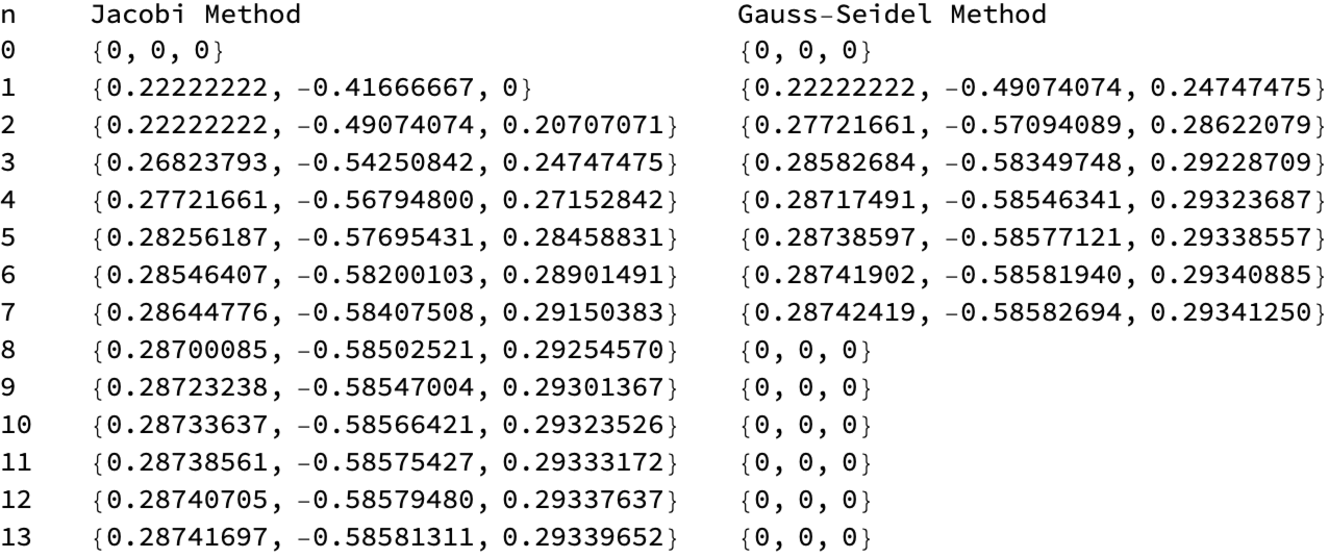
\includegraphics[scale=0.65]{hw5q1p1}

\begin{mmaCell}{Output}

\end{mmaCell}
\vspace{-5pt}\h9\h9\h9\h9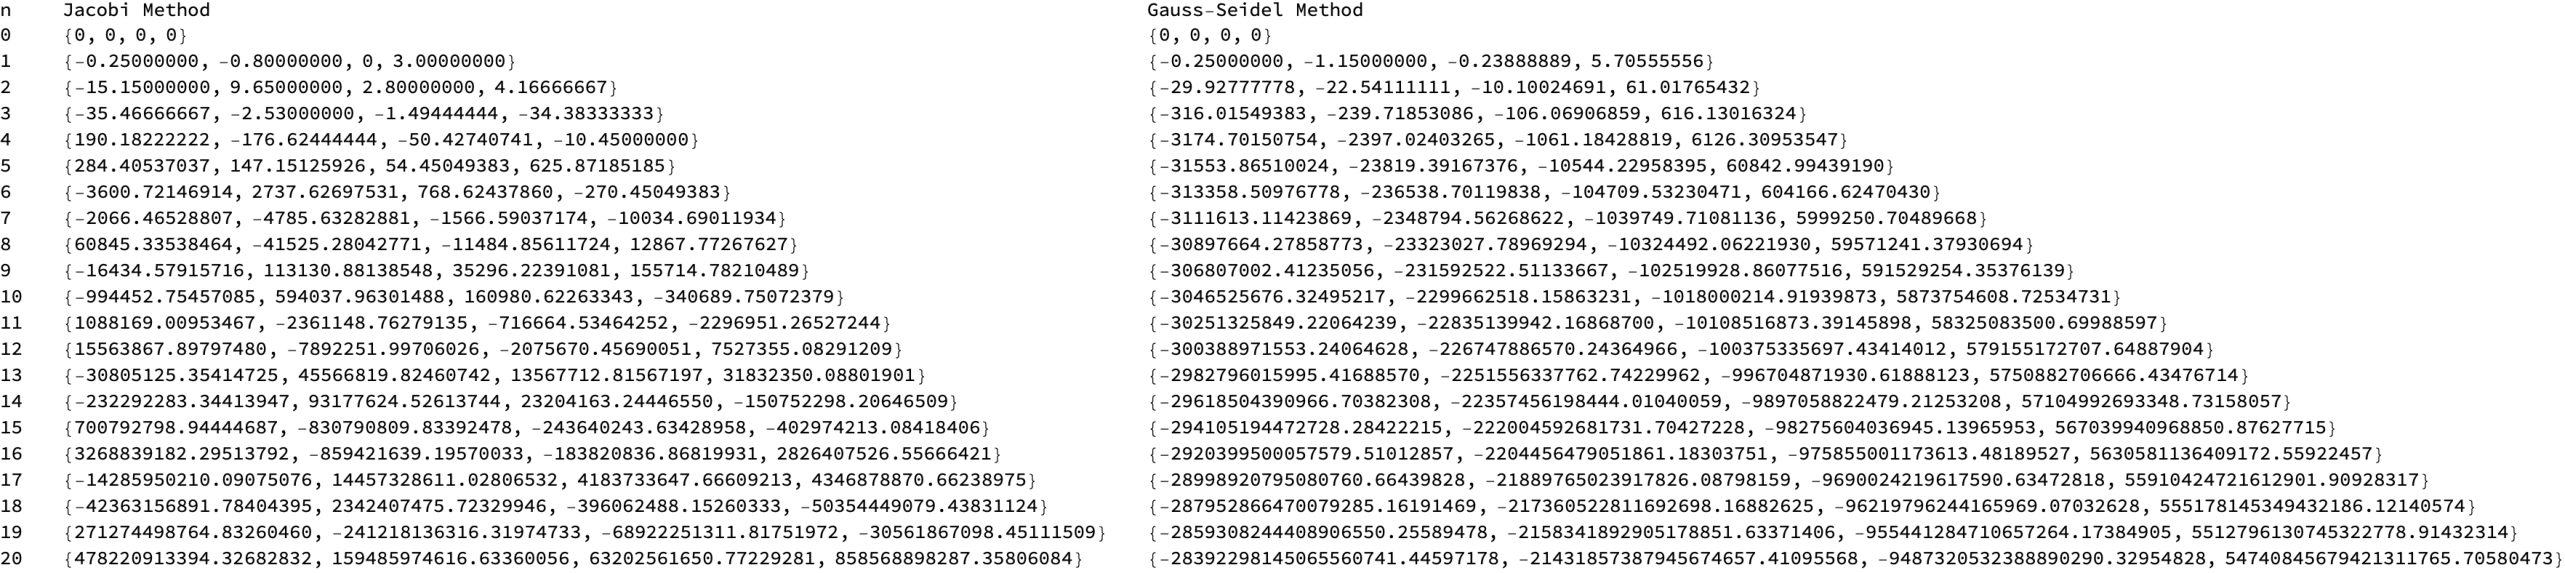
\includegraphics[scale=0.35]{hw5q1p3}

\newpage
\begin{mmaCell}{Output}

\end{mmaCell}
\vspace{-5pt}\h9\h9\h9\h9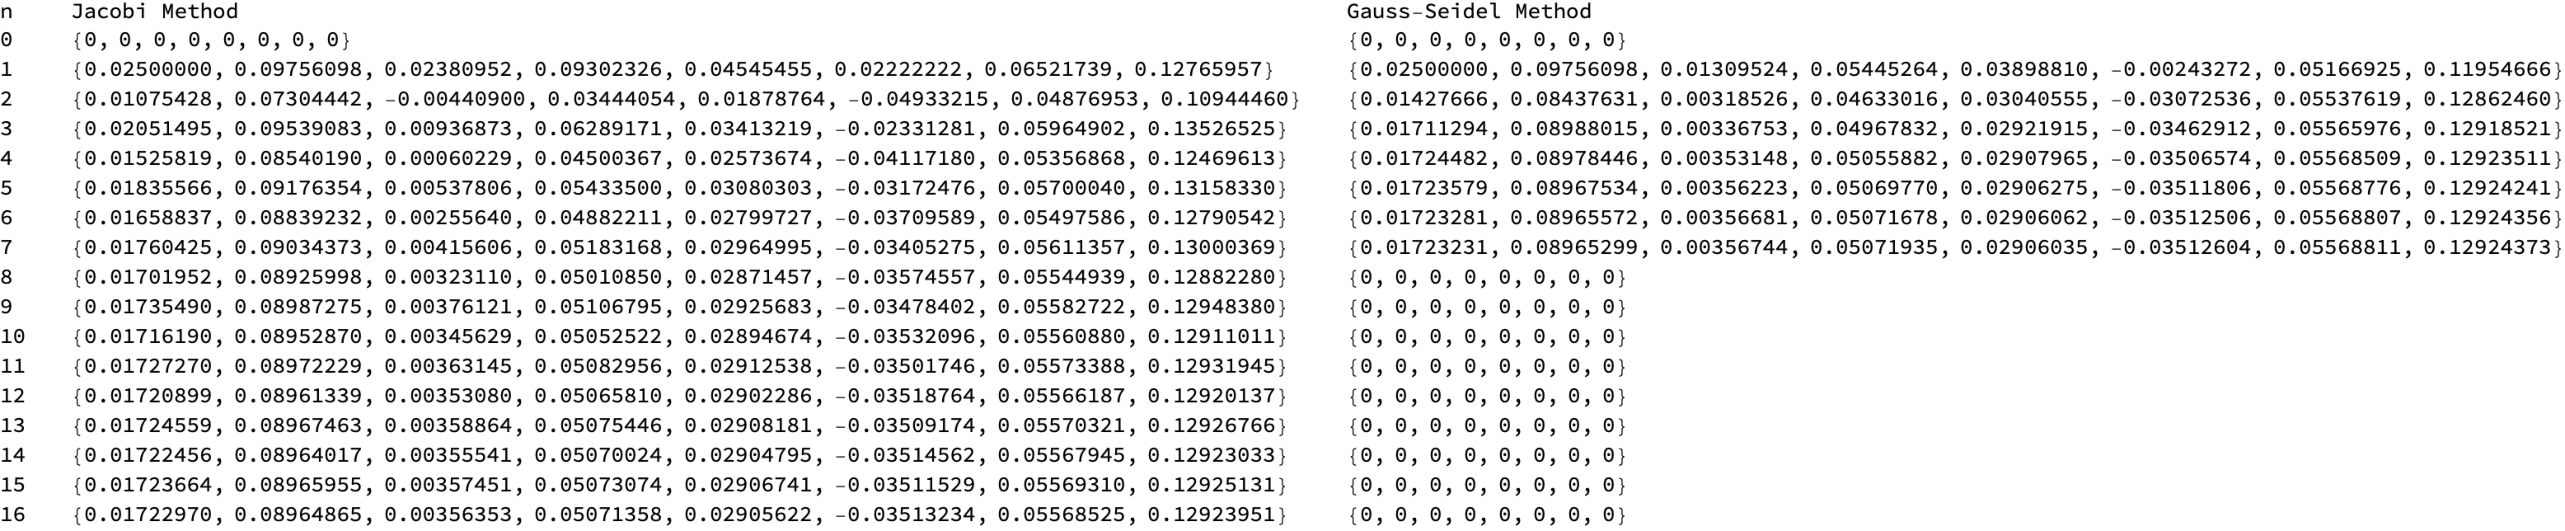
\includegraphics[scale=0.35]{hw5q1p4}

\vspace{10pt}
\noindent I didn't include the matrix from (ii) because it was crashing my Mathematica. Let $\mathbf{x},\mathbf{b} \in \bbC^n$ and $A \in \Mat_{n}(\bbC)$. Recall that the iterative formula for the Jacobi method is:
    \begin{equation*}
    \begin{split}
        \mathbf{x}^{(k+1)} = D^{-1} \left( \mathbf{b} - (L + U)\mathbf{x}^{(k)} \right),
    \end{split}
    \end{equation*}
where $A = D + L + U$, that is, it is decomposed into a diagonal, strictly lower triangular, and strictly upper triangular matrix. Similarly, The iterative formula for the Gauss-Seidel method is:
    \begin{equation*}
    \begin{split}
        \mathbf{x}^{(k+1)} = L^{-1}(\mathbf{b} - U \mathbf{x}^{(k)}),
    \end{split}
    \end{equation*}
where $A = L + U$, that is, it is decomposed into a lower triangular and strictly upper triangular matrix. For part (ii), we can clearly see that $\det(D^{-1}) = 0$ and $\det(L^{-1}) = 0$, implying the matrix cannot be inverted. Mathematica doesn't like this.

Recall $A \in \Mat_{n}(\bfC)$ is \textit{invertible} if there exists a $B \in \Mat_{n}(\bfC)$ such that $AB = BA = I_n$. For $A \in \Mat_{n,m}(\bfC)$, a \textit{pseudoinverse} of $A$ is a matrix $A^+ \in \Mat_{m,n}(\bfC)$ satisfying the following properties:
    \begin{enumerate}[label = (\arabic*),itemsep=1pt,topsep=3pt]
        \item $A A^+ A = A$;
        \item $A^+ A A^+ = A$;
        \item $(A A^+)^\ast = A A^+$;
        \item $(A^+ A)^\ast = A^+ A$,
    \end{enumerate}
where $\square^\ast$ denotes the conjugate transpose. Replacing each instance of \texttt{Inverse[]} with \texttt{PseudoInverse[]} in the above code, we have:
\newpage

\begin{mmaCell}[functionlocal=y]{Code}
CompareJacobiGauss[A2, b2, x2]
\end{mmaCell}
\begin{mmaCell}{Output}
    
\end{mmaCell}
\vspace{-5pt}\h9\h9\h9\h9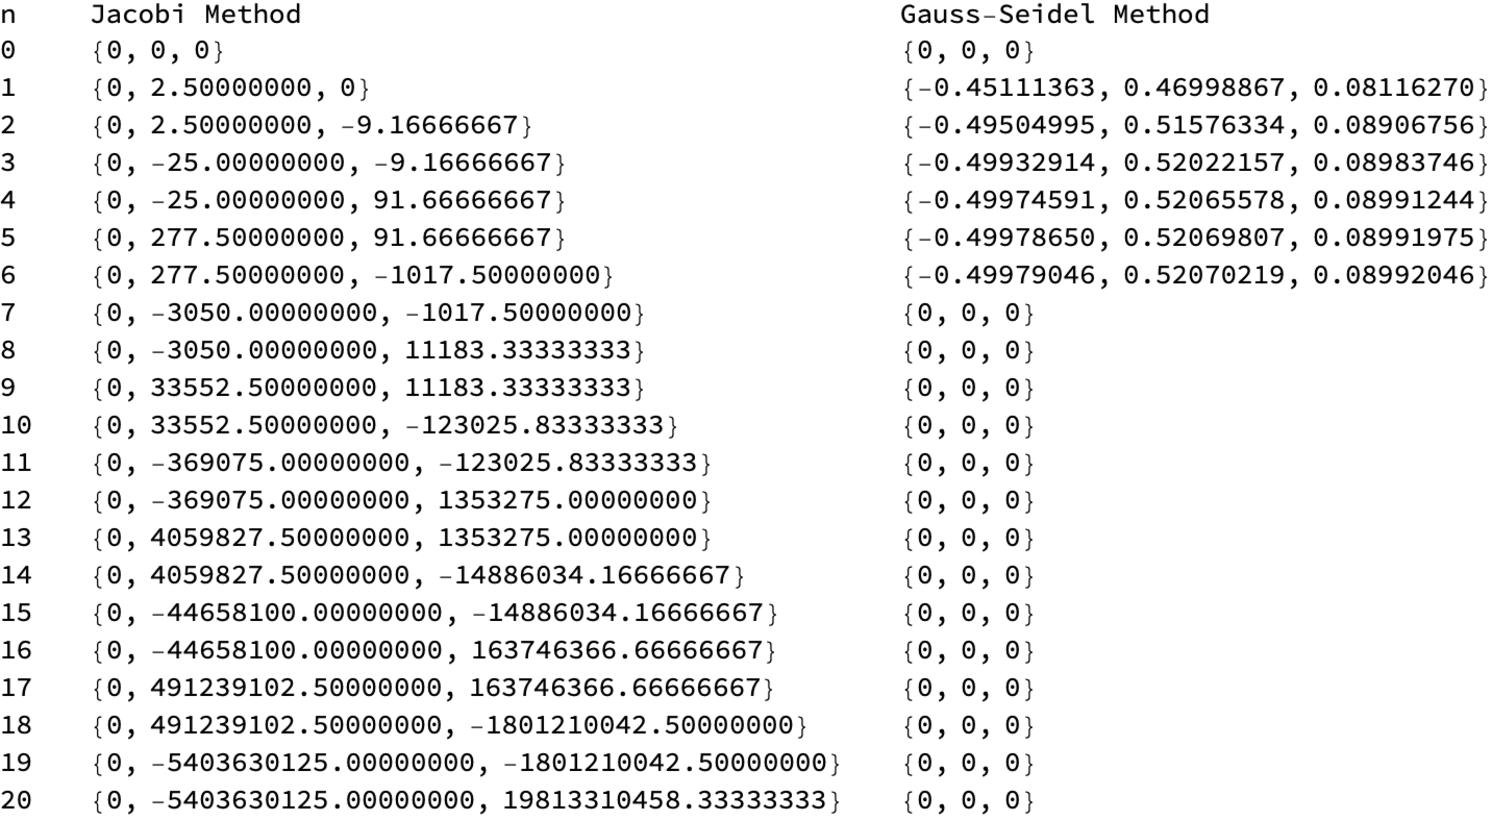
\includegraphics[scale=0.58]{hw5q1p2.pdf}

\noindent Neither the Jacobi method nor the Gauss-Seidel method converged to a correct solution, but it's still cool nonetheless!
%%%%%%%%%%%%%%%%%%%%%%%%%%%%%%%%%%%%%%%%%%%%%%%%%%%%%%%%%%%%%
\vspace{25pt}

\noindent (c) I wrote the code below to do parts (i), (ii), and (iii). From the table at the very end, the rate at which the absolute errors change is approximately linear.

\begin{mmaCell}[functionlocal=y]{Code}
Clear["Global`*"]
EulersMethod[f_, leftEndpoint_, rightEndpoint_, deltaX_, 
   initialCondition_] := 
  Module[{a, b, h, x, y, yVals, n, points, plot},
   a = leftEndpoint;
   b = rightEndpoint;
   h = deltaX;
   x = Table[x, {x, a, b, h}];
   y = Table[0, {Length[x]}];
   y[[1]] = initialCondition;
   For[n = 1, n < Length[x], n++, 
    y[[n + 1]] = N[y[[n]] + h*f[x[[n]], y[[n]]], 10];];
   points = Transpose[{x, y}];
   plot = ListLinePlot[points, PlotRange -> All];
   {MatrixForm[points], plot, points}
   ];

f[x_, y_] := x*y^2 + x^2*y - 2;
p1 = EulersMethod[f, 0, 2, 1, 1];
p2 = EulersMethod[f, 0, 2, 1/2, 1];
p3 = EulersMethod[f, 0, 2, 1/4, 1];
p4 = EulersMethod[f, 0, 2, 1/8, 1];
p5 = EulersMethod[f, 0, 2, 1/16, 1];
{p1[[1]], p1[[2]]}
{p2[[1]], p2[[2]]}
{p3[[1]], p3[[2]]}
{p4[[1]], p4[[2]]}
{p5[[1]], p5[[2]]}
ListLinePlot[{p1[[3]], p2[[3]], p3[[3]], p4[[3]], p5[[3]]}, 
 PlotLabel -> "y'[x] = x*y^2+x^2*y-2", PlotRange -> All, 
 PlotLegends -> {"h=1", "h=1/2", "h=1/4", "h=1/8", "h=1/16"}]

g[x_, y_] := -8*y + Sin[x];
q1 = EulersMethod[g, 0, 2, 1, 0];
q2 = EulersMethod[g, 0, 2, 1/2, 0];
q3 = EulersMethod[g, 0, 2, 1/4, 0];
q4 = EulersMethod[g, 0, 2, 1/8, 0];
q5 = EulersMethod[g, 0, 2, 1/16, 0];
{q1[[1]], q1[[2]]}
{q2[[1]], q2[[2]]}
{q3[[1]], q3[[2]]}
{q4[[1]], q4[[2]]}
{q5[[1]], q5[[2]]}
ListLinePlot[{q1[[3]], q2[[3]], q3[[3]], q4[[3]], q5[[3]]}, 
 PlotLabel -> "y'[x] = -8*y +Sin[x]", PlotRange -> All, 
 PlotLegends -> {"h=1", "h=1/2", "h=1/4", "h=1/8", "h=1/16"}]

h[x_, y_] := y *Cos[x];
r1 = EulersMethod[h, 0, 2, 1, 2];
r2 = EulersMethod[h, 0, 2, 1/2, 2];
r3 = EulersMethod[h, 0, 2, 1/4, 2];
r4 = EulersMethod[h, 0, 2, 1/8, 2];
r5 = EulersMethod[h, 0, 2, 1/16, 2];
{r1[[1]], r1[[2]]}
{r2[[1]], r2[[2]]}
{r3[[1]], r3[[2]]}
{r4[[1]], r4[[2]]}
{r5[[1]], r5[[2]]}
ListLinePlot[{r1[[3]], r2[[3]], r3[[3]], r4[[3]], r5[[3]]}, 
 PlotLabel -> "y'[x] = y*Cos[x]", PlotRange -> All, 
 PlotLegends -> {"h=1", "h=1/2", "h=1/4", "h=1/8", "h=1/16"}]

y[x_] := 2 Exp[Sin[x]];
delta = {1, 1/2, 1/4, 1/8, 1/16};
approx = {r1[[3, -1, 2]], r2[[3, -1, 2]], r3[[3, -1, 2]], 
   r4[[3, -1, 2]], r5[[3, -1, 2]]};
errors = {Abs[approx[[1]] - y[2]], Abs[approx[[2]] - y[2]], 
   Abs[approx[[3]] - y[2]], Abs[approx[[4]] - y[2]], 
   Abs[approx[[5]] - y[2]]};
table = Table[{
    delta[[n]],
    approx[[n]],
    errors[[n]]
    }, {n, 1, Length[delta]}];
TableForm[
 Prepend[table, {"deltaX", "y_{approx}[2]", "|y_{approx}[2] - y_{exact}[2]|"}]]
\end{mmaCell}
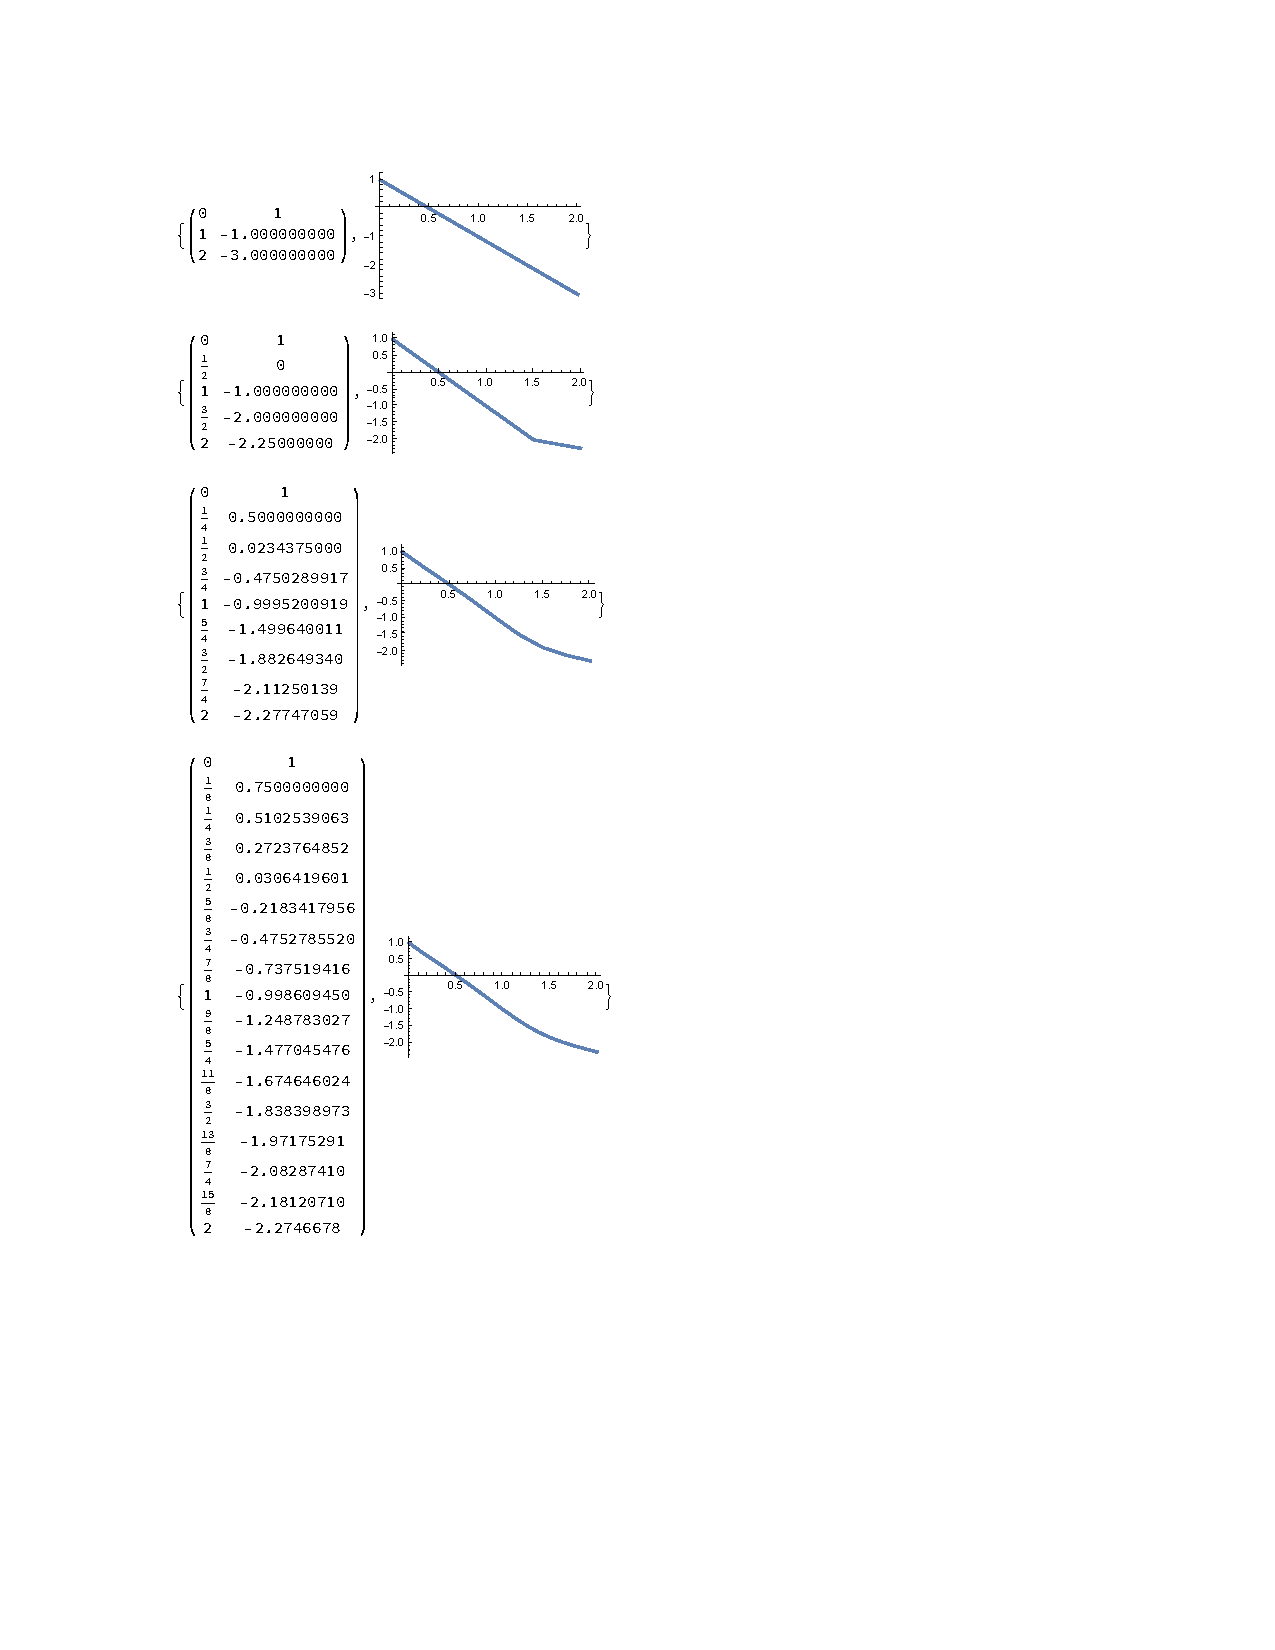
\includepdf[pages=-]{blah3}

%%%%%%%%%%%%%%%%%%%%%%%%%%%%%%%%%%%%%%%%%%%%%%%%%%%%%%%%%%%%%
\end{document}